\documentclass[UTF8]{article}
\usepackage{bm}
\usepackage{amsmath}
\usepackage{cases}
\usepackage{cite}
\usepackage{graphicx}
\usepackage[margin=1in]{geometry}
\geometry{a4paper}
\usepackage{fancyhdr}
\pagestyle{fancy}
\usepackage{wrapfig}
\fancyhf{}
\usepackage{float}  %设置图片浮动位置的宏包
\usepackage{subfigure}
\usepackage{caption}
\usepackage{booktabs}
\usepackage{listings}
\usepackage{xcolor}
\lstset{numbers=left, %设置行号位置
	numberstyle=\tiny, %设置行号大小
	keywordstyle=\color{blue}, %设置关键字颜色
	commentstyle=\color[cmyk]{1,0,1,0}, %设置注释颜色
	frame=single, %设置边框格式
	escapeinside=``, %逃逸字符(1左面的键),用于显示中文
	breaklines, %自动折行
	extendedchars=false, %解决代码跨页时,章节标题,页眉等汉字不显示的问题
	xleftmargin=2em,xrightmargin=2em, aboveskip=1em, %设置边距
	tabsize=4, %设置tab空格数
	showspaces=false %不显示空格
}

\title{Measurement of the thermal conductivity of non-good conductors}
\author{by 22 Artificial Intelligence ChenxuZhang}
\date{2023.3.29}
\pagenumbering{arabic}

\begin{document}
	
	\fancyhead[L]{ChenxuZhang}
	\fancyhead[R]{ID 202264691028}
	\fancyfoot[C]{\thepage}
	
	\maketitle
	\tableofcontents
	\newpage
	
	\section{Abstract}
The thermal conductivity of a material is an important parameter reflecting its thermal conductivity, and it directly measures the thermal insulation performance of the material. The manufacture of melting furnaces,heat transfer pipes, radiators, heaters, etc. all take into account the thermal conductivity of the material. Therefore, the study and measurement of the thermal conductivity of materials is necessary. Materials with a high thermal conductivity and good thermal conductivity are called good conductors of heat, while the opposite is true for poor conductors of heat. In general, the thermal conductivity of metals is greater than that of non-metals, that of solids is greater than that of liquids, and that of gases is the smallest. Because the thermal conductivity of a material changes not only with temperature and pressure, but also with the impurity content and structure of the material, the thermal conductivity of a material is often determined experimentally in scientific experiments and engineering techniques. The methods of measuring thermal conductivity can be broadly divided into two types: the steady state method and the dynamic method. The steady state method is often used in teaching experiments to measure the thermal conductivity of non-good conductors. The steady state method is a simple, visual, accurate and reliable method of measurement and is mainly suitable for measurements at low and medium temperatures.\\
	\textbf{Result:}Based on the experimental results, we calculated the thermal conductivity of the sample to be tested as:$\lambda  =  1.7645\times 10^{-4} \left ( W\cdot m^{-1}\cdot ^{\circ}C^{-1}    \right )$From the experimental data, it is clear that silicone rubber has a smaller thermal conductivity, poorer thermal conductivity and better insulation properties, making it suitable as an insulation material.
	\\
	\textbf{Key Words: Bad conductor, Thermal conductivity, Least squares, Steady state method, Heat transfer}
	
	
	\section{Purpose of the experiment}
   $\bm{A}$.Learn about the co-axial adjustment of simple optical systems.\\
   $\bm{B}$.Learn several ways to measure the focal length of convex and concave lenses.\\
   $\bm{C}$.Experiment with ways to measure the focal length of thin lenses and deepen your understanding of the principles of optical imaging.\\
   $\bm{D}$.Understand the principles of optical imaging and the thin lens formula.
      

	\section{Experimental apparatus}
	
		\subsection{Optical Instruments Group}
		The optical instrument set consists of the following items: optical tool holders, convex lenses, concave lenses, parallel white light sources, sodium lamps, object screens, pincushion screens, flat reflectors, etc.
		
		\begin{figure}[H]
			\centering
			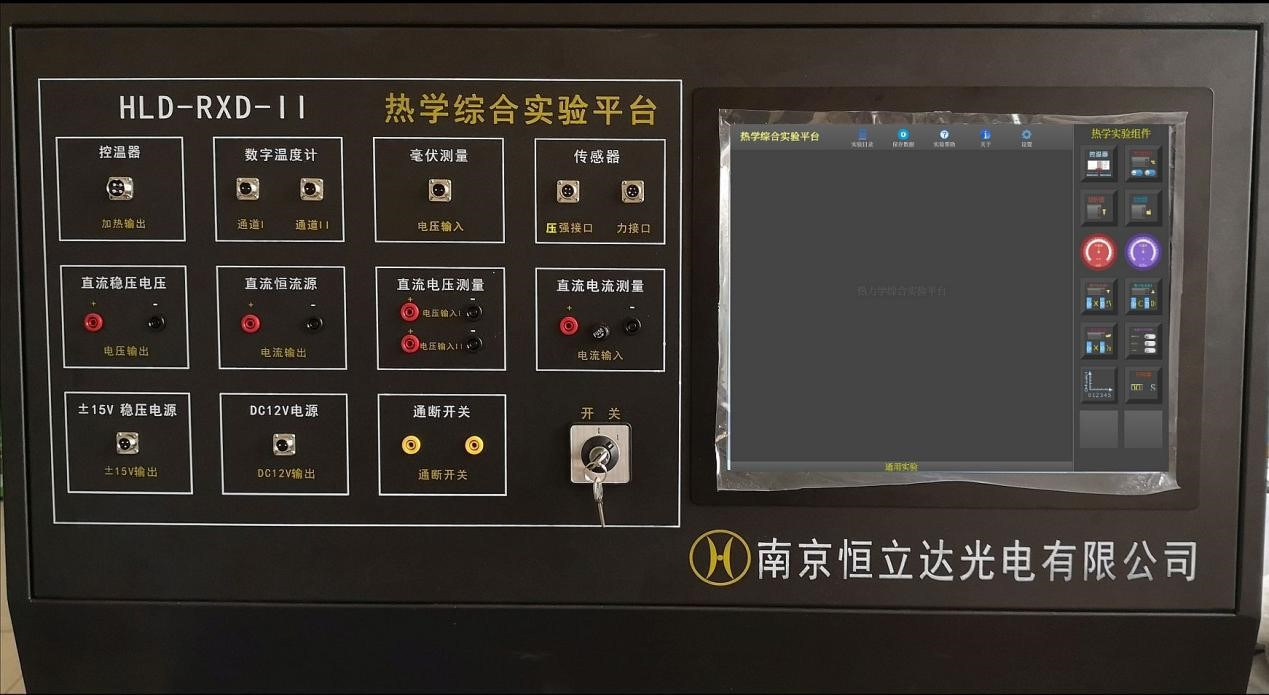
\includegraphics[clip,scale=0.9,trim={0 50 0 30}]{fig/fig3.jpg}
			\caption{Host panel}
			\label{figure.1}
		\end{figure}
		\begin{figure}[H]
			\begin{minipage}[t]{0.5\linewidth}
				\centering
				
\includegraphics[clip,scale=0.6,trim={0 4 0 4}]{fig/fig1.png}
				\caption{Basic Interface}
				\label{figure.2}
			\end{minipage}
			\begin{minipage}[t]{0.5\linewidth}
				\centering
				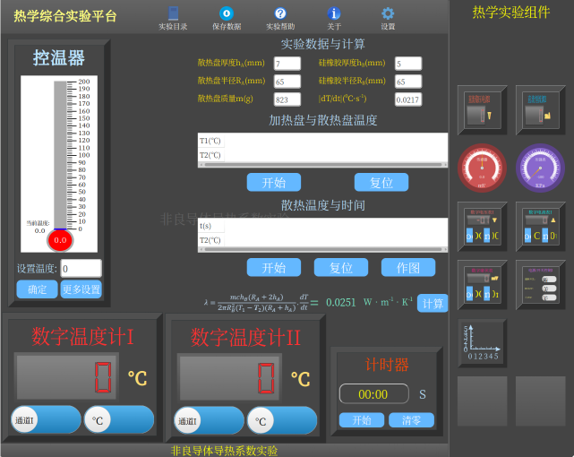
\includegraphics[clip,scale=0.5]{fig/fig2.png}
				\caption{The interface after opening the component}
				\label{figure.3}
			\end{minipage}
		\end{figure}
	    
	 

	    \subsection{Thermal conductivity test accessories and samples to be tested}
	    The thermal conductivity test accessories include a temperature-controlled heating device (which contains a heated metal plate and a fan), two temperature probes (one end of which is connected to the test platform and the other to the metal plate), gloves and protective cream. The temperature-controlled heating unit is used to control the heating temperature to maintain a constant temperature, the temperature probes measure the temperature of the upper and lower metal plates in real time, the gloves are used to protect the experimenter's hands from burns when removing the sample to be tested and the protective cream is applied to the upper and lower surfaces of the sample to be tested to protect the sample.
	    \begin{figure}[H]
	    	\begin{minipage}[t]{0.4\linewidth}
	    		\centering
	    		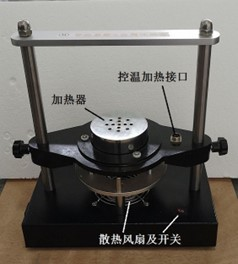
\includegraphics[clip,scale=0.8,trim={0 4 0 4}]{fig/fig4.jpg}
	    		\caption{ Thermal conductivity test accessories}
	    		\label{figure.4}
	    	\end{minipage}
	    	\begin{minipage}[t]{0.65\linewidth}
	    		\centering
	    		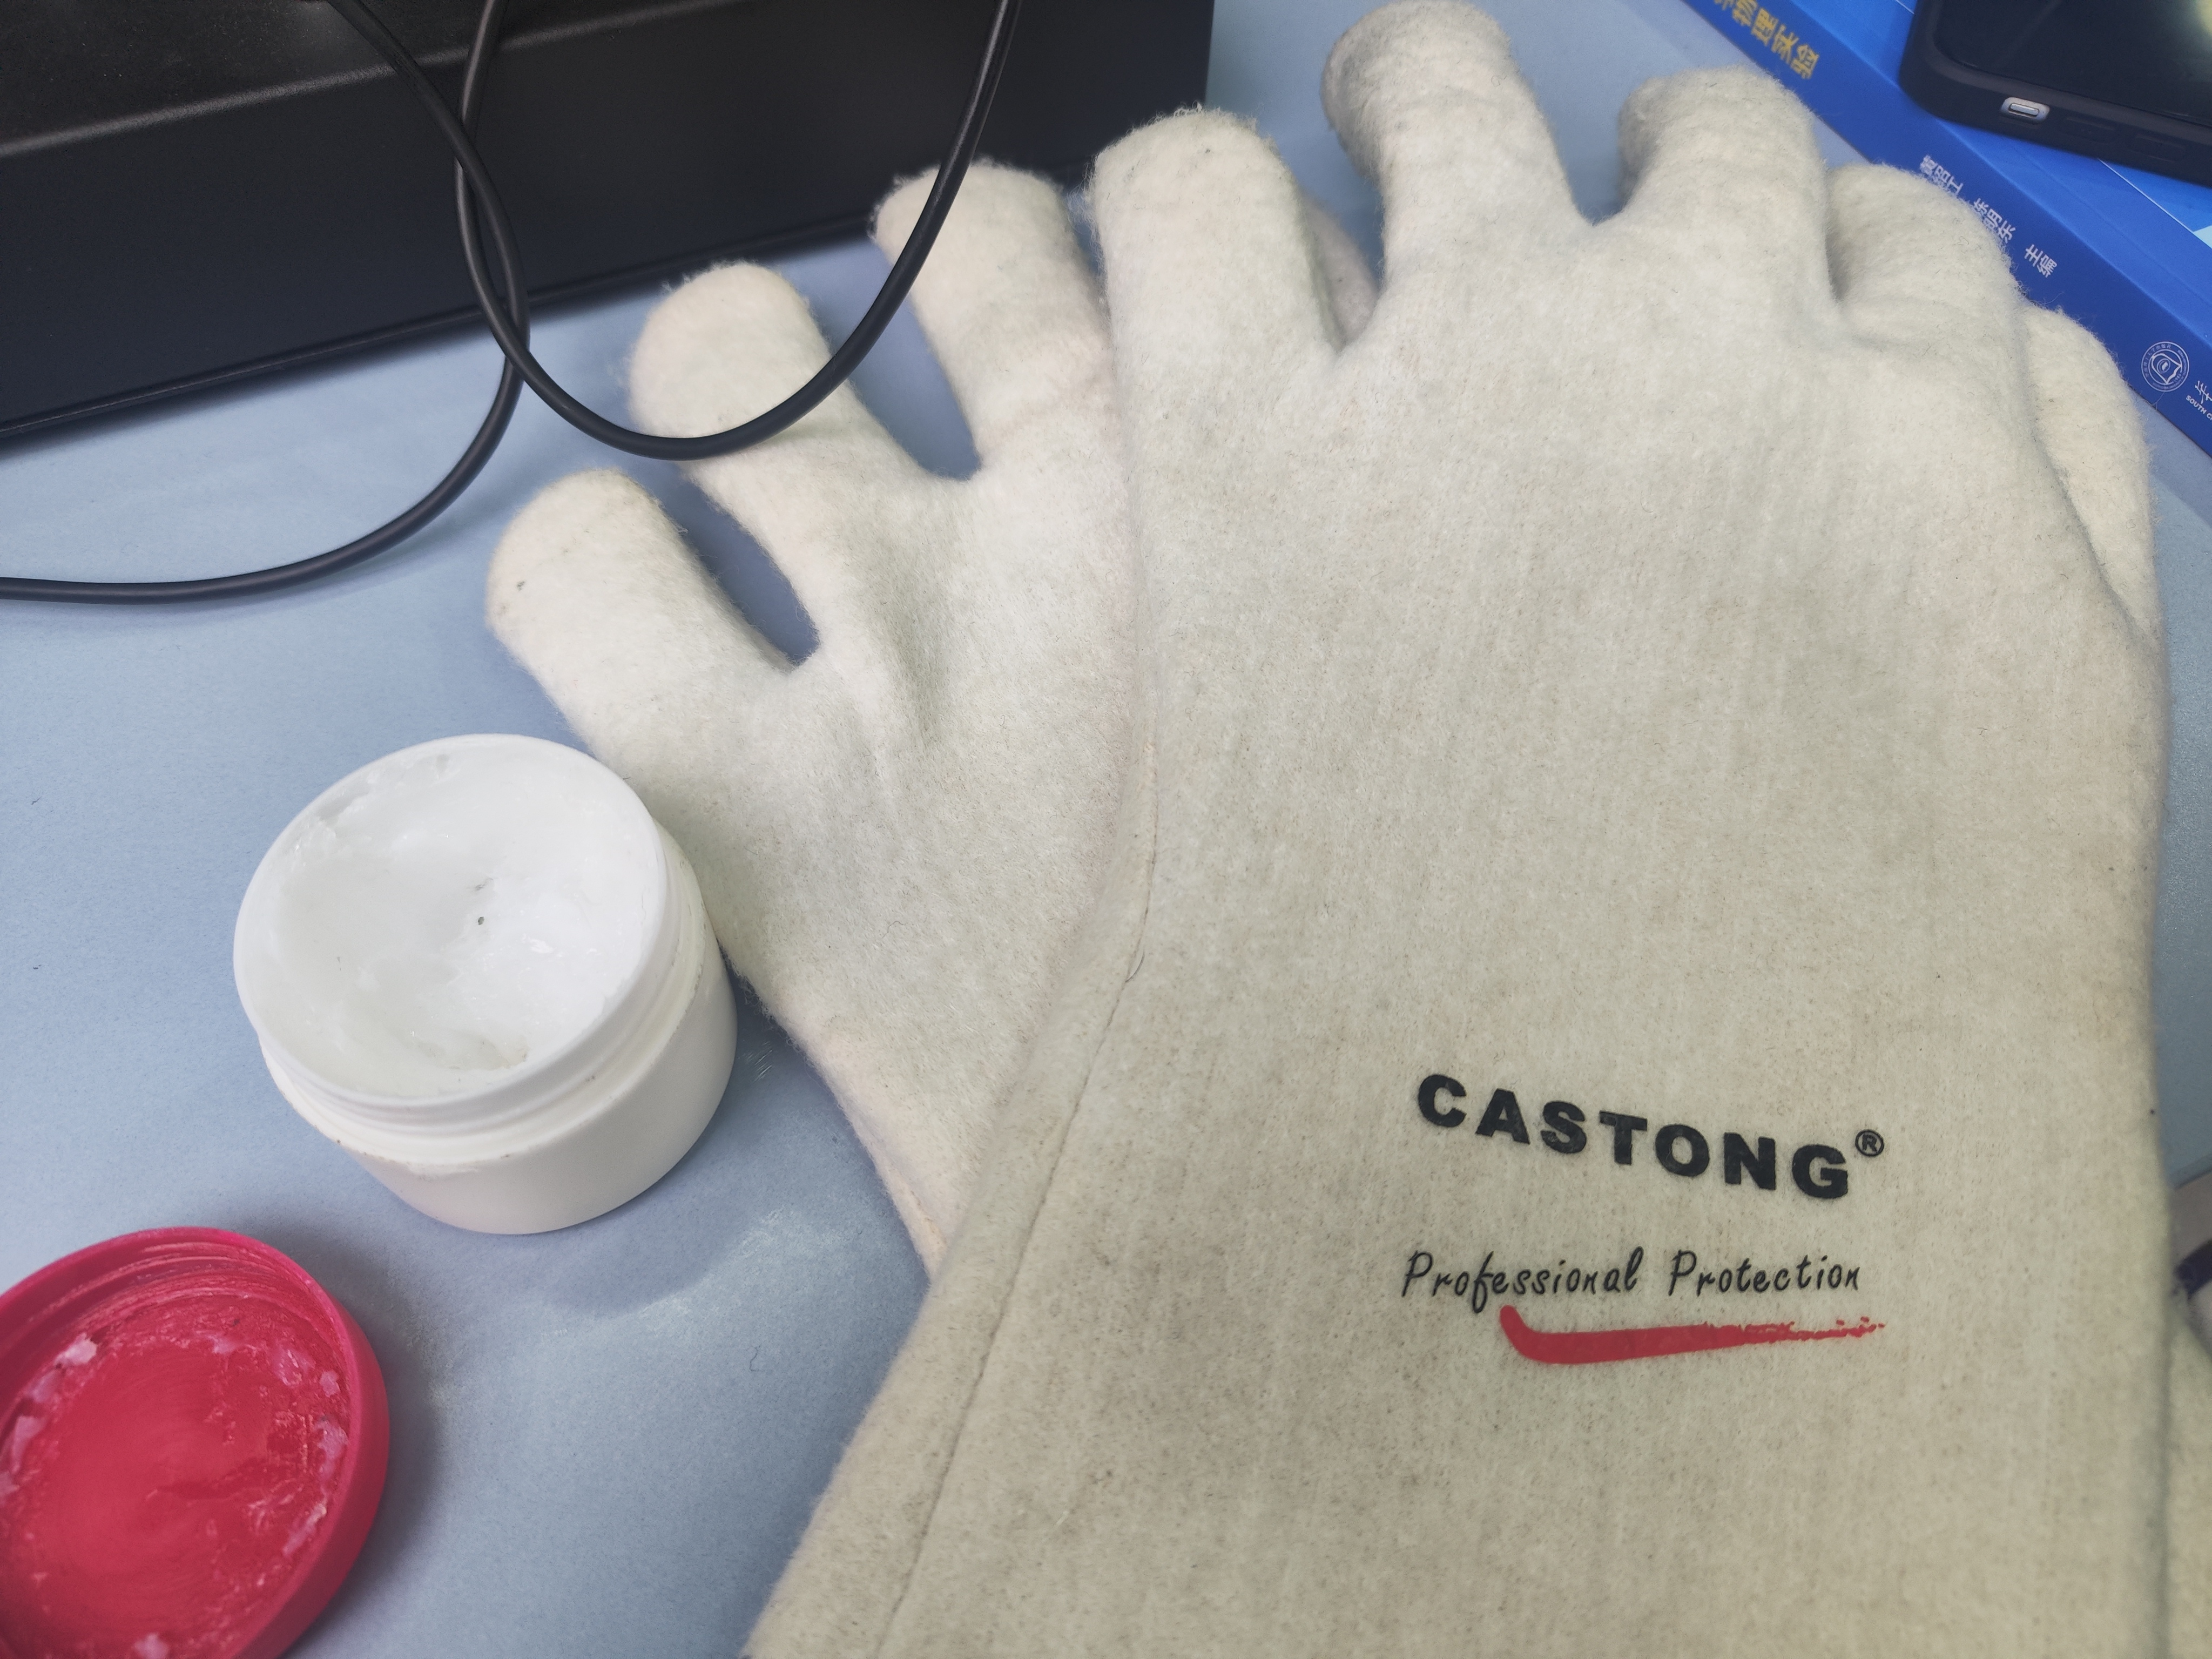
\includegraphics[clip,scale=0.07,trim={400 0 100 120}]{fig/fig5.jpg}
	    		\caption{TGloves and protective cream}
	    		\label{figure.5}
	    	\end{minipage}
	    \end{figure}
    
       The sample to be tested for the experiment, a pancake shaped piece of silicone rubber, is a typical poor conductor of electricity. For the experiments, we heated it using upper and lower metal discs clamped to its upper and lower surfaces.
       \begin{figure}[H]
      	\centering
      	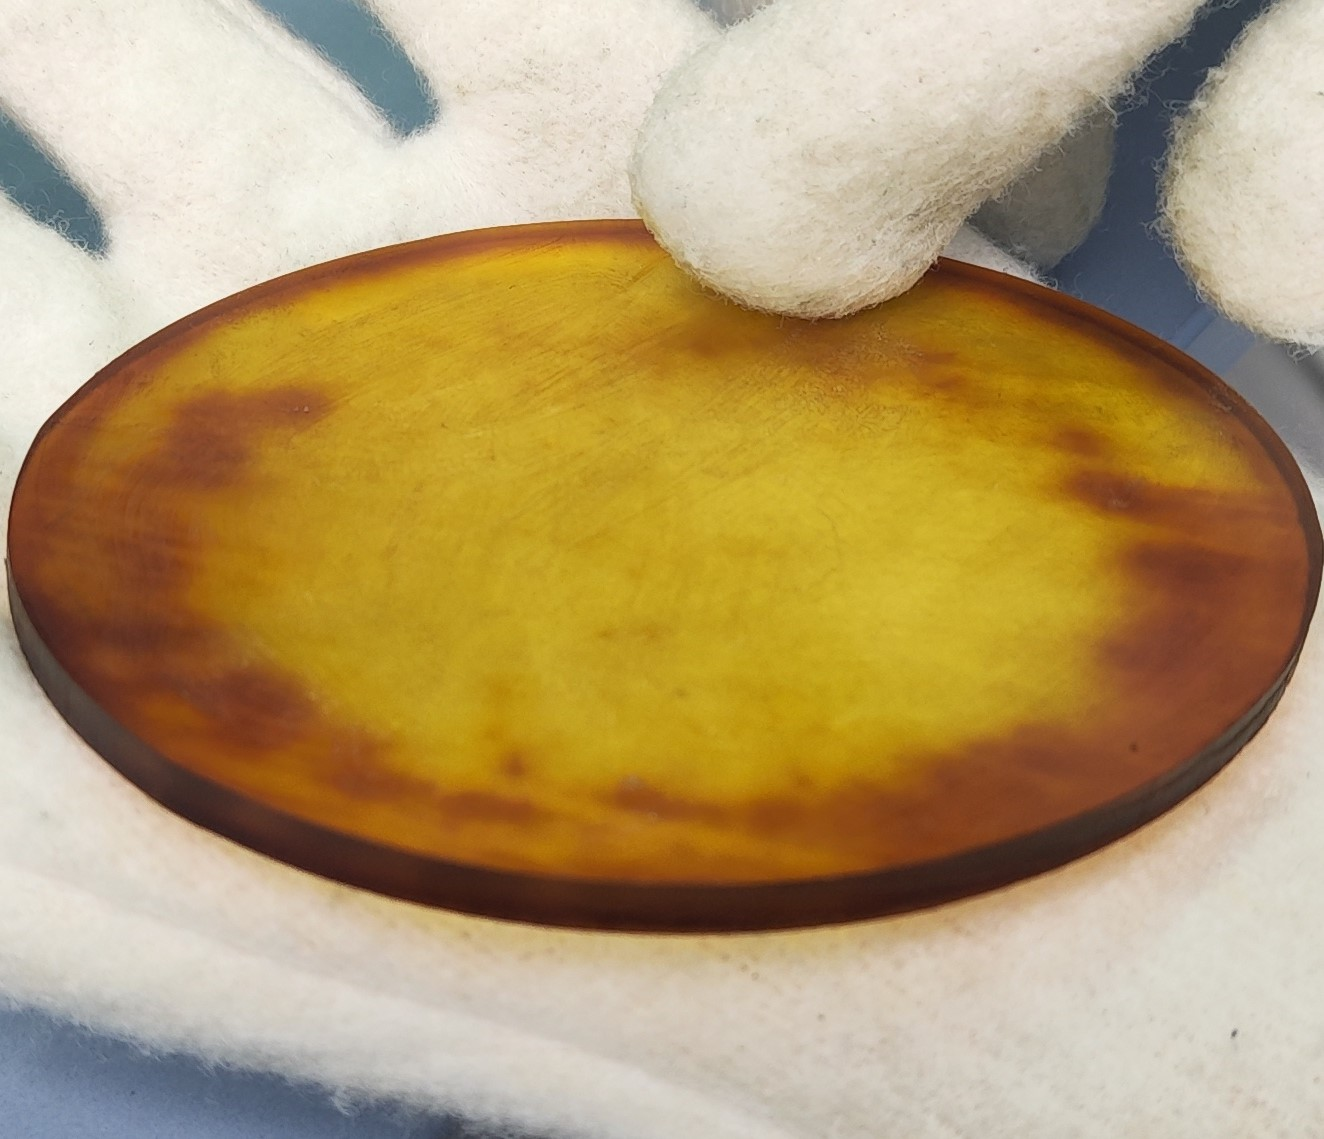
\includegraphics[clip,scale=0.25,trim={0 210 0 200}]{fig/fig6.jpg}
      	\caption{The sample to be tested}
      	\label{figure.6}
      \end{figure}
      
	\section{Experimental principles}
    As early as 1882, the French scientist Fourier formulated the law of heat conduction and various methods of measuring thermal conductivity are now based on Fourier's law. Fourier's law of heat conduction is the basis for all current methods of measuring thermal conductivity.
    
    when the temperature is not uniform throughout the interior of an object, there is a flow of heat from the higher temperature areas to the lower temperature areas.  This phenomenon is known as heat conduction. The law of heat conduction states that if heat is transferred in the Z-direction, then by taking a vertical section $dS$ at any location $Z_{0} $ on the Z-axis and expressing the temperature gradient in $\frac{dT}{dZ}$ at Z in $^{\circ} C\cdot m^{-1} $, and expressing the rate of heat transfer (heat per unit time through the cross-sectional area dS) in $W$ at that location in $\frac{dQ}{dt} $, then the law of heat conduction can be expressed as:
    \begin{eqnarray}dQ & = & -\lambda \left ( \frac{dT}{dz} \right )_{z_{0} }  ds\cdot dt\end{eqnarray}
    
    The negative sign in the equation indicates that the heat is flowing from the high temperature region to the low temperature region (i.e. the direction of heat transfer is opposite to the direction of the temperature gradient) and the proportionality factor $\lambda $ is the coefficient of thermal conductivity in $W\cdot m^{-1}\cdot ^{\circ}C^{-1} $. It can be seen that the physical meaning of the coefficient of thermal conductivity is the amount of heat perpendicularly passing through a unit cross-sectional area per unit time for a temperature gradient of one unit. Using equation (1) to measure the thermal conductivity $\lambda $ of a material, two key issues need to be addressed: one is how to create a temperature gradient $\frac{dT}{dZ}$ within the material and determine its value; the other is how to measure the rate of heat transfer from the high temperature region to the low temperature region within the material $\frac{dQ}{dt} $.
    
	\subsection{Determination of temperature $\frac{dT}{dZ}$}
    In order to create a temperature gradient distribution within the sample, the sample can be machined into a flat plate and sandwiched between two good conductors.The upper and lower plates are maintained at constant temperatures $T_{1}$ and $T_{2}$ respectively, creating a temperature gradient in the direction perpendicular to the sample surface.The temperature gradient is distributed in the direction perpendicular to the sample surface. If the sample thickness $h$ is much smaller than the sample diameter $D\left (h\ll D  \right ) $, the sample side surface area is much smaller than its upper and lower surface area and the heat dissipated by the sides is negligible and the heat can be considered to flow in the direction perpendicular to the upper and lower surfaces of the sample, i.e. there is a temperature gradient only in this direction. Since copper is a good conductor of heat, at equilibrium it can be assumed that the temperature is the same everywhere on the same copper plate and everywhere on the same parallel plane within the sample. Thus, by measuring the thickness $h$ of the sample and the temperatures $T_{1}$ and $T_{2}$ of the two copper plates, the temperature gradient within the sample can be determined as:
    
    \begin{eqnarray}\frac{dT}{dZ} & = & \frac{T_{1}-T_{2}  }{h} \end{eqnarray}
    
    This of course requires the copper plate to be in close contact with the sample surface without gaps, otherwise the air layer in between will create thermal resistance and make the temperature gradient measurement inaccurate. In addition, to ensure a good symmetry in the distribution of the temperature field in the sample, the sample and the two copper plates are machined into equal circles.
    
    \begin{figure}[H]
    	\centering
    	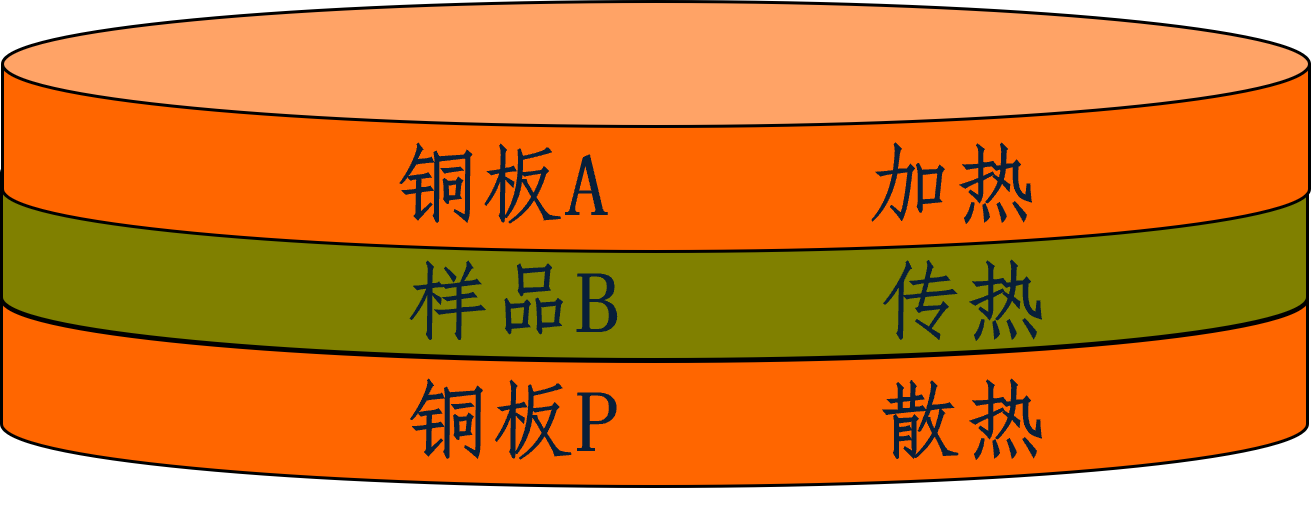
\includegraphics[clip,scale=0.8]{fig/fig8.png}
    	\caption{Operation diagram}
    	\label{figure.7}
    \end{figure}
    
	\subsection{Determination of heat transfer rate $\frac{dQ}{dt} $}
	
	\begin{wrapfigure}{r}{5.5cm}%靠文字内容的左侧
		\centering
		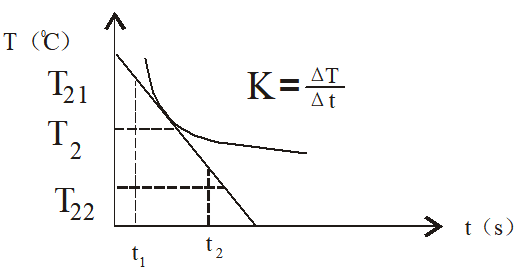
\includegraphics[width=0.4\textwidth,trim={0 35 0 0}]{fig/fig9.png}
		\caption{\footnotesize $\left ( T\sim t \right ) $ graph}
	\end{wrapfigure}

	The amount of heat $\frac{dQ}{dt} $ passing through a certain cross-sectional area per unit of time is a quantity that cannot be directly measured and we have managed to convert this quantity into a more easily measurable one. In order to maintain a constant temperature gradient distribution, the high temperature side of the copper plate must be continuously heated, the heat is transferred through the sample to the low temperature side of the plate, and the low temperature side of the plate has to continuously dissipate heat to the surroundings. When the heating rate, heat transfer rate and heat dissipation rate is equal, the system will reach a dynamic equilibrium, called steady state. At this point the rate of heat dissipation from the low temperature side of the copper plate is the rate of heat transfer within the sample. Thus, by measuring the heat dissipation rate of the copper plate at the steady state temperature $T_{2}$, the heat transfer rate within the sample is also indirectly measured. However, the heat dissipation rate of the copper plate is not easy to measure and further parametric conversion is required. We know that the heat dissipation rate of a copper plate is related to the cooling rate (rate of change in temperature) $\frac{dT}{dt} $, which is expressed as:
	
	\begin{eqnarray}\left. \frac{\text{d}Q}{\text{d}t} \right|_{T=T_2}=-\left. m_{\text{A}}c\frac{\text{d}T}{\text{d}t} \right|_{T=T_2} \end{eqnarray}
	
	Where mA is the mass of the copper plate and c is the specific heat capacity of the copper plate, with the negative sign indicating the transfer of heat to the low temperature direction. Since the mass is easily measured directly and c is a constant, the measurement of the heat dissipation rate of the copper plate is then transformed into a measurement of the cooling rate of the copper plate on the low temperature side. The cooling rate of the copper plate can be measured in this way: after the temperature of the upper and lower plates has reached a stable level, the sample is removed and the upper plate is heated directly against the lower plate so that the temperature of the lower plate is higher than the steady-state temperature $T_{2}$ (approximately $10^{\circ} C$ higher) and then allowed to cool naturally in the environment until the temperature is below T2, the temperature is measured in the interval from greater than $T_{2}$ to less than T2 with time and the $\left ( T\sim t \right ) $ curve is plotted. The slope of the curve at $T_{2}$ is the cooling rate of the copper plate at steady state temperature at $T_{2}$. (It should be noted that the resulting $\frac{dT}{dt}$ is the cooling rate of the entire surface of the copper plate exposed to air, with a heat dissipation area of $2\Pi R_{A} ^{2} +2\Pi R_{A}h_{A} $ where $R_{A}$ and $h_{A}$ are the radius and thickness of the lower copper plate, respectively). Let the radius of the sample cross-section be $R_{A}$ , and in the experiment for steady-state heat transfer, the upper surface of the lower copper plate (area of $2\Pi R_{A} ^{2}$ is covered by all of the sample $\left ( R_{B}=R_{A} \right ) $, and since the cooling rate of objects is proportional to their area, the expression for the cooling rate of the copper plate in steady state should be modified to:
	
	\begin{eqnarray}\frac{dQ}{dt} & = & -m_{A} c\frac{dT}{dt}  \cdot \frac{\pi R_{A} ^{2} +2\pi R_{A}h_{A}}{2\pi R_{A} ^{2} +2\pi R_{A}h_{A}} \end{eqnarray}

	\subsection{Formula derivation}
    In order to calculate the thermal conductivity 1234, we need to bring equation (2) and equation (4) into equation (1), and we have no difficulty in obtaining the following equation:
    
    \begin{eqnarray}\lambda  =  -m_{A}c\frac{R_{A}+2h_{A}  }{2R_{A}+2h_{A}}  \cdot \frac{1}{\pi R_{B}^2 }\cdot \frac{h_{A} }{T_{1}-T_{2}  }\cdot\left. \frac{dT}{dt} \right| _{T  =  T_{2} }    \end{eqnarray}
    
   According to the above formula, we can calculate the result by putting the data obtained through the experiment into the calculation formula.

	\section{Contents and Steps}
	
	\begin{itemize}
		\item After connecting the cables according to the wiring diagram shown in Figure 10, turn on the power supply of the experimental platform (just turn the key in the lower right corner of the platform to the open position).
		\item On the platform interface, select "Thermal Conductivity of Non-Good Conductors Experiment" under "Experimental Catalogue", then drag out the thermometer I, thermometer II, and timer modules from the "Thermal Experimental Components" on the right-hand side, Timer Module, Power/Switch Control. Set "DC12V" on the power/switch control to "on".
		\item Measure the radius $R_{B}$ and thickness $B_{h}$ of the sample B to be measured, the radius $R_{A}$ and thickness $A_{h}$ of the heat sink A and the mass $m_{A}$. thickness $A_{h}$ and mass $m_{A}$, noting the units.
		\item Place the sample to be tested, B, between the heating plate C and the heat sink A. Adjust the three fine adjustment screws on the bracket of the heat sink A so that B is in good contact with A and C. Insert the temperature probes into the small holes in the sides of A and C, to the bottom of the holes, so that the temperature probes are in good contact with the copper tray.A corresponds to temperature channel I, C to temperature channel II.
	\end{itemize}
     
     \begin{figure}[H]
     	\begin{minipage}[t]{0.5\linewidth}
     		\centering
     		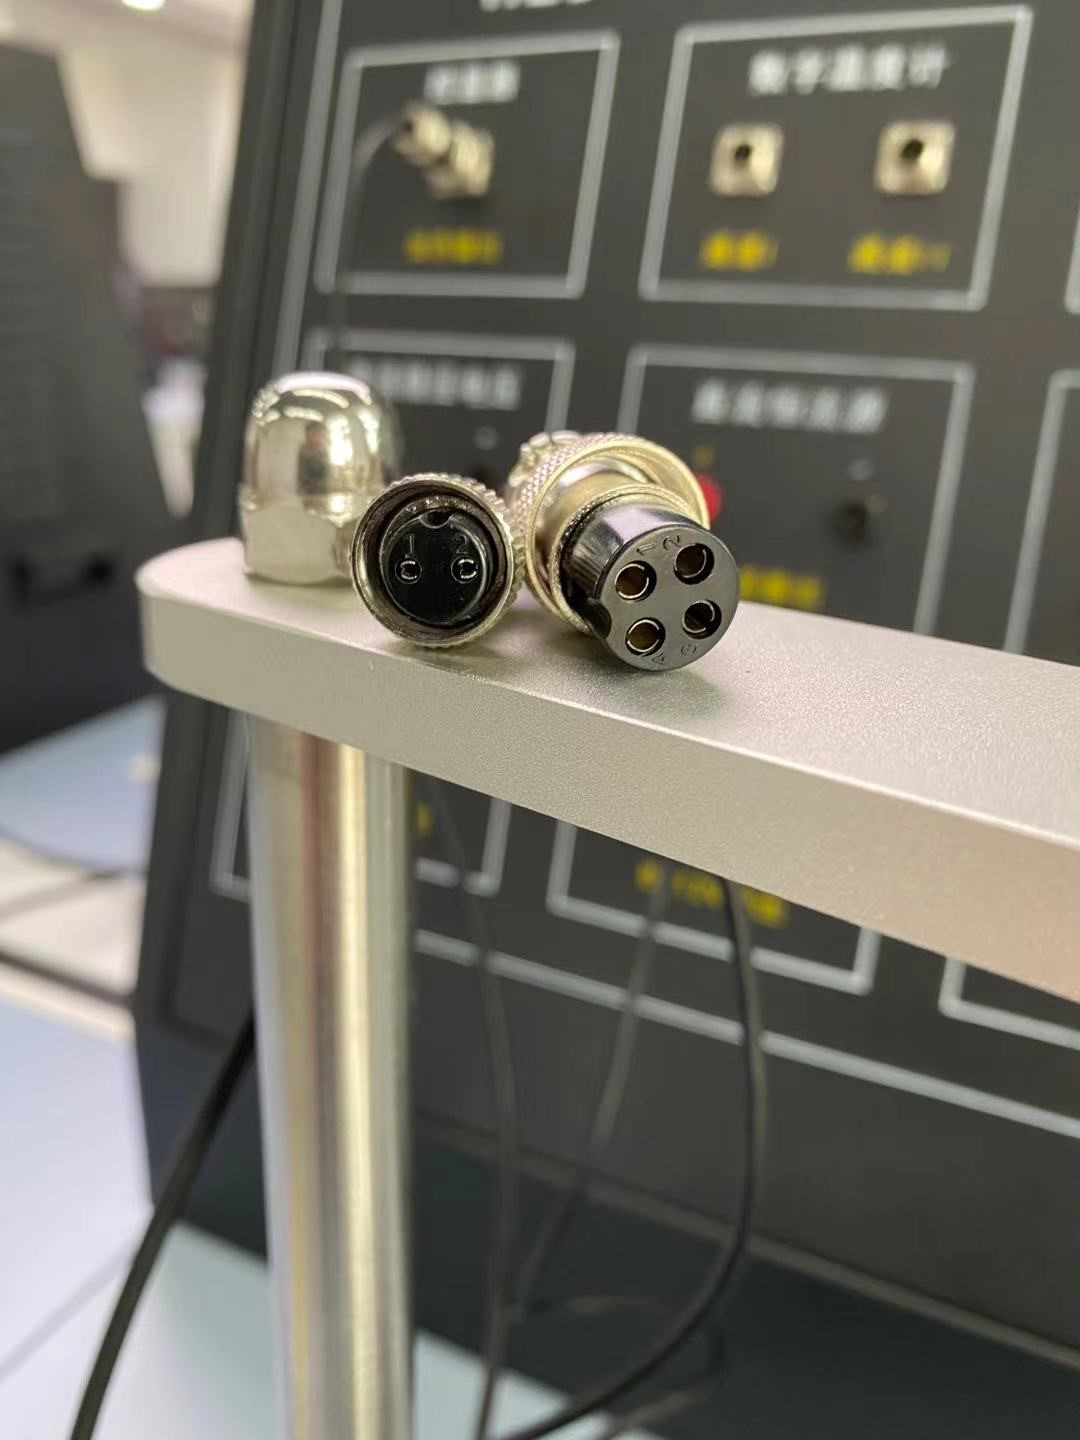
\includegraphics[clip,scale=0.195,trim={0 4 0 4}]{fig/fig7.jpg}
     		\caption{ Connectors}
     		\label{figure.8}
     	\end{minipage}
     	\begin{minipage}[t]{0.5\linewidth}
     		\centering
     		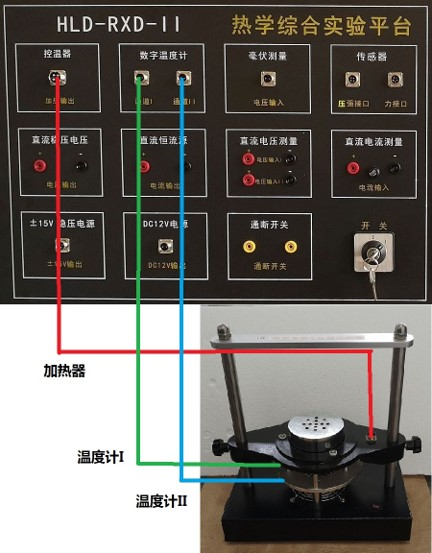
\includegraphics[clip,scale=0.5]{fig/fig10.jpg}
     		\caption{Wiring method}
     		\label{figure.9}
     	\end{minipage}
     \end{figure}
	\begin{itemize}
		\item Set the thermostat temperature to $80^{\circ} C$ and click the "Start" button on the platform interface under the table for recording the temperature of the heating plate and the cooling plate, the system will record the temperature of heating plate C $T_{1}$ and cooling plate A $T_{2}$ every 60 seconds.
		\item Allow a long time for the system to reach a stable temperature distribution. After the system has been heated for a period of time (approx. 40 minutes) and after the $T_{1}$ reading has stabilised (less than $0.2^{\circ} C$ fluctuation), record the temperature values in Table 2 every 2 minutes until the $T_{2}$ value does not change significantly (less than 0.2 fluctuation in 10 minutes) and stop recording
		\item Measure the heat dissipation rate of the heat sink A around the stable temperature value $T_{2}$ $\frac{dQ}{dt} $: Remove C, remove B and bring C into direct contact with A. When the temperature of A rises to about $10^{\circ} C$ above the $T_{2}$ value, remove C again and expose all surfaces of A to the air. Allow A to cool naturally and start recording the heat dissipation temperature and time in Table 3 until the temperature drops below a certain value of $T_{2}$ and stop recording.
		\item The $\left ( T\sim t \right ) $ cooling rate curve for the copper disc is calculated by selecting the measurement data adjacent to $T_{2}$ to find the cooling rate and entering it into the input box to calculate the thermal conductivity $\lambda $ of the sample.
	\end{itemize}
     \begin{figure}[H]
     	\centering
     	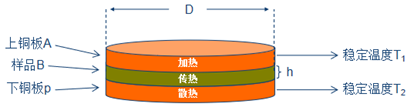
\includegraphics[clip,scale=1.1]{fig/fig11.png}
     	\caption{Operation diagram}
     	\label{figure.10}
     \end{figure}
    
	
	\section{Data processing}
	To measure the cooling rate of the copper plate, after the temperature of the upper and lower copper plates reach stability, remove the sample and use the upper copper plate to heat the lower copper plate.
	\subsection{Basic data measurement and recording}
    First, we measure the heat sink and the sample to be tested. Here we measure several times and then average the values of the multiple measurements and record them in Table 1. The data recorded includes the thickness of the heat sink, the radius of the heat sink, the mass of the heat sink, the thickness of the sample to be tested and the radius of the sample to be tested:
    	\begin{table}[H]
    		\centering
    	\begin{tabular}{cccc}
    		\toprule
    		 & the thickness h$\left (mm \right ) $ & radius R$\left ( mm  \right ) $&mass M$\left (g \right ) $\\
    		\midrule
    		the heat sink & 7.00 & 65.00 & 823.00 \\
    		the sample to be tested & 5.00 & 65.00 & null \\
    		\bottomrule
    	\end{tabular}
    \caption{Basic data measurement and recording}
    \label{table.1}
    \end{table}

    \subsection{Stable temperature measurement}
    After the system has been heated for approximately 40 minutes, record the upper and lower copper plate temperatures every 2 minutes from the time the $T_{1}$ $\left ( ^{\circ} C \right ) $ reading is stable until the $T_{2}$ $\left ( ^{\circ} C \right ) $ reading is also relatively stable. Record the temperature readings of the upper and lower copper plates every 2 minutes,Shown in Table 2:
    
    \begin{table}[H]
    	\centering
    	\begin{tabular}{ccccccccccc}
    		\toprule
    		& 1st & 2ed & 3rd & 4th & 5th & 6th & 7th &8th & 9th & 10th \\
    		\midrule
    		$T_{1}$ $\left ( ^{\circ} C \right ) $ & 80.2 & 80.3 & 80.3 & 80.3 & 80.2 & 80.0 & 79.7 & 78.4 & 78.3 & 78.5\\
    		$T_{2}$ $\left ( ^{\circ} C \right ) $ & 59.7 & 60.1 & 60.5 & 60.7 & 60.9 & 61.1 & 61.2 & 61.3 & 61.4 & 61.2\\
    		\bottomrule
    	\end{tabular}
    	\caption{Stable temperature measurement}
    	\label{table.2}
    \end{table}
    
    To ensure the authenticity of the experimental data, we have included actual photographs of the data in the \textbf{appendix}.
    
    Next we plotted the graphs for the data as above:
     \begin{figure}[H]
    	\centering
    	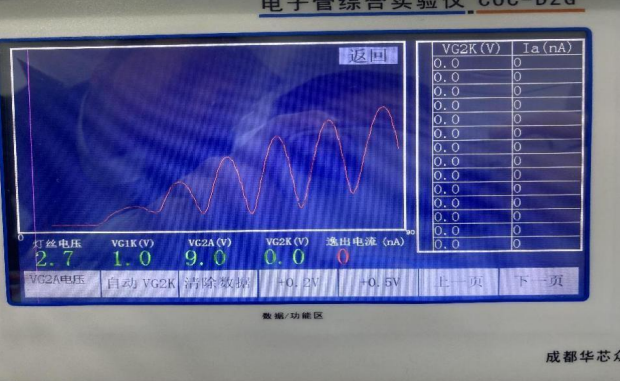
\includegraphics[clip,scale=0.8]{fig/fig12.png}
    	\caption{$T_{2} \sim t$Relationship icons}
    	\label{figure.11}
    \end{figure}
    
    It is easy to see from the graph that $T_{2}$ tends to rise overall with time and stabilises once the rise reaches $61.2^{\circ} C$ degrees. So, we can tell that when the upper metal plate is controlled at around $80.0^{\circ} C$, the lower metal plate reaches a constant state at around $61.2^{\circ} C$. Therefore, we record the data at this point and obtain a constant temperature of $61.2^{\circ} C$:
    
    \begin{eqnarray}T_{1} & = & 80.0\end{eqnarray}
    \begin{eqnarray}T_{2} & = & 61.2\end{eqnarray}
    
    \subsection{Heat dissipation rate measurement}
    Measure the rate of heat dissipation from the lower copper plate around the steady state value $T_{2}$. When the lower copper plate is cooling naturally, record the temperature indication every 30s as shown in the table below:
    
    \begin{table}[H]
    	\centering
    	\begin{tabular}{ccccccccccccccc}
    		\toprule
    		& 1st & 2ed & 3rd & 4th & 5th & 6th & 7th &8th & 9th & 10th & 11th & 12th & 13th & 14th\\
    		\midrule
    		t$\left ( second \right ) $ & 30 & 60 & 90 & 120 & 150 & 180 & 210 & 240 & 270 & 300 & 330 & 360 & 390 & 420\\
    		$T_{2}$ $\left ( ^{\circ} C \right ) $ & 70.4 & 68.4 & 66.4 & 64.6 & 62.9 & 61.4 & 59.9 & 58.5 & 57.2 & 55.9 & 54.6 & 53.4 & 52.3 & 51.2\\
    		\bottomrule
    	\end{tabular}
    	\caption{Stable temperature measurement}
    	\label{table.3}
    \end{table}

   Based on the above data, we tried to draw the relation curve of $T_{2} \sim t$. We considered using curves to fit the data. After consulting the data, we found that $T_{2} \sim t$ presented an inverse proportional relationship, so we tried to fit the curve on this basis:
    
   \begin{figure}[H]
   	\centering
   	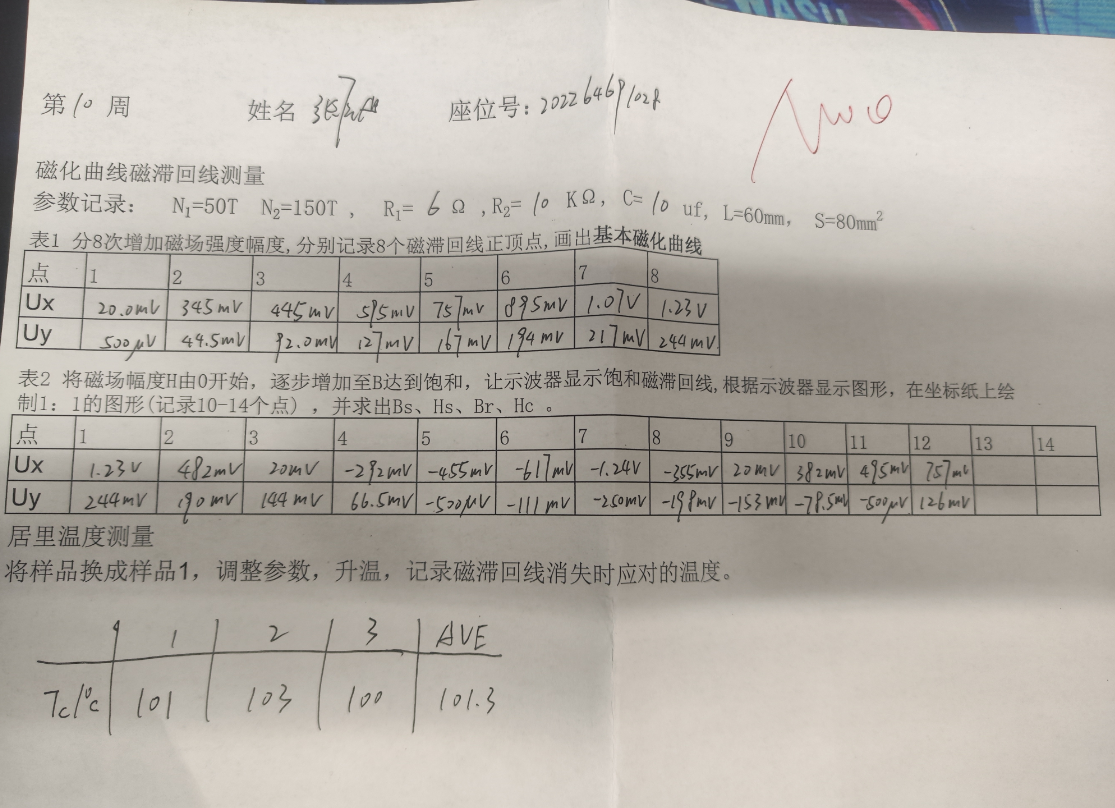
\includegraphics[clip,scale=0.7]{fig/fig13.png}
   	\caption{$T_{2} \sim t$Relationship icons}
   	\label{figure.12}
   \end{figure}
	
	We can see that in the interval around the constant temperature of $T_{2}$ (10 degrees Celsius left and right), $T_{2}$ varies in an approximately straight line, but there is still some curvature. We suspect that this is because the span of the horizontal coordinates is so large that it is difficult to present a clear inverse proportional image. At the same time, the image also shows that the cooling temperature of $T_{2}$ as a function of time is generally consistent with the standard.

    \subsection{Data extraction and calculation of results}
    According to the equation, we also need to calculate the ratio of the temperature of the metal disc with time at the moment $T_{2}$. We therefore combine the curve in Figure 13 and find the tangent line to the curve at the moment $T_{2}$, we calculate the slope of the tangent line and write it down as:
     \begin{figure}[H]
    	\centering
    	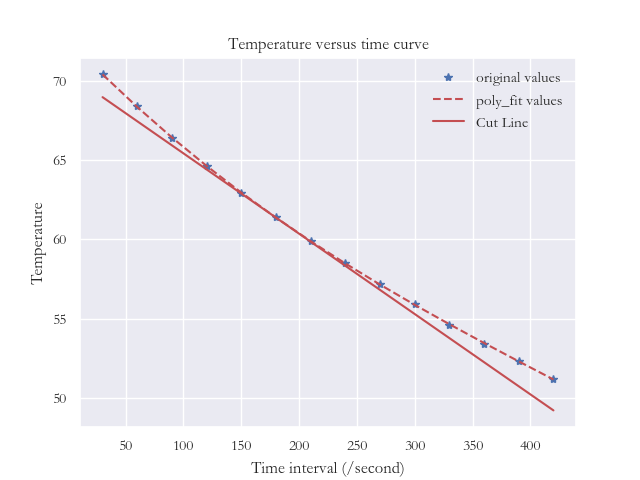
\includegraphics[clip,scale=0.75]{fig/fig14.png}
    	\caption{$T_{2}$ curve}
    	\label{figure.13}
    \end{figure}

     Also, we obtain the equation for the tangent line as follows:
     
     \begin{eqnarray}y  =  -0.05066x+70.48999\end{eqnarray}
     \begin{eqnarray}\frac{dT_{2} }{dt} & = & -0.05066\left ( ^{\circ}C\cdot s^{-1}   \right ) \end{eqnarray}
     
     Finally, by bringing the above data into the equation, we can calculate the thermal conductivity of the sample to be measured:
     
     \begin{eqnarray}\lambda  =  -m_{A}c\frac{R_{A}+2h_{A}  }{2R_{A}+2h_{A}}  \cdot \frac{1}{\pi R_{B}^2 }\cdot \frac{h_{A} }{T_{1}-T_{2}  }\cdot\left. \frac{dT}{dt} \right| _{T  =  T_{2} }    \end{eqnarray}
     \begin{eqnarray} & = & 1.7645\times 10^{-4} \left ( W\cdot m^{-1}\cdot ^{\circ}C^{-1}    \right ) \end{eqnarray}
    
\section{Conclusion and analysis}
\subsection{Experimental conclusion}

Based on the experimental results, we calculated the thermal conductivity of the sample to be tested as:

\begin{eqnarray}\lambda & = & 1.7645\times 10^{-4} \left ( W\cdot m^{-1}\cdot ^{\circ}C^{-1}    \right ) \end{eqnarray}

From the experimental data, it is clear that silicone rubber has a smaller thermal conductivity, poorer thermal conductivity and better insulation properties, making it suitable as an insulation material.

\subsection{Experimental error analysis}
	\begin{itemize}
	\item The thermal conductivity should be measured in such a way that $T_{1}$ and $T_{2}$ are in a steady state, i.e. the two temperatures remain constant for ten minutes and $\left ( T_{2}< T_{1}   \right ) $. The cooling rate around $T_{2}$ should be measured in the experiment.
	\item When the heat sink is at different temperatures, it dissipates heat at different rates, related to the body temperature and the ambient temperature. In the experiment, when the system is in steady state, the heat transfer through the sample to be tested is at the same rate as the heat sink to the side and below, so the cooling rate is measured around the steady state temperature $T_{2}$,。
	\item Fans work to increase air flow, intensifying heat transfer and forcing convection with a much larger heat dissipation coefficient than natural convection. If the fan does not work, the heat dissipation does not reach the required level and the measured heat dissipation rate is not accurate.
\end{itemize}

\begin{appendix}
	\section{Documentation of experimental procedures}
	\begin{figure}[H]
		\centering
		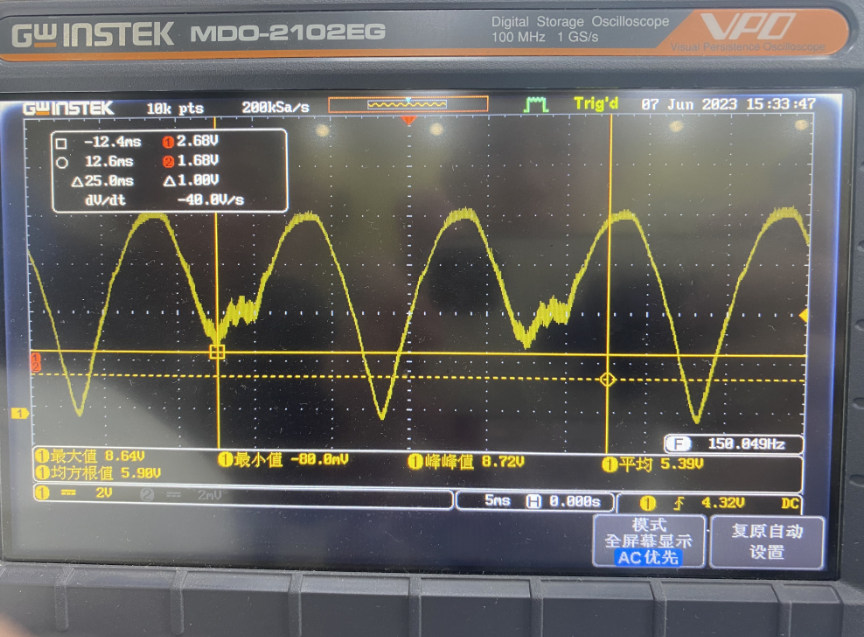
\includegraphics[clip,scale=0.08]{fig/fig15.jpg}
		\caption{Experimental data proves}
		\label{figure.14}
	\end{figure}
	
	\section{Data Analysis and Visualisation Source Code}
	\begin{lstlisting}[language=python]
import seaborn as sns
import pandas as pd
import numpy as np
from matplotlib import pyplot as plt
#=======================================
#Image background settings
plt.style.use('seaborn-darkgrid')
sns.set(style = 'darkgrid')
import  warnings
warnings.filterwarnings('ignore')
plt.rcParams['font.sans-serif'] = ['STSong']
#=======================================
#Calculating tangents
def numerical_diff(f, x):
    h = 1e-7
    return (f(x + h) - f(x - h)) / (2 * h)
#Constructed tangents
def tangent_line(f, x):
    d = numerical_diff(f, x)
    y = f(x) - d * x
    print(y,d)
    return lambda t: d * t + y
#Read data
file1 = pd.read_excel('./data/data2.xlsx')
#=========================================
x = file1['a']
y = file1['b']
z1 = np.polyfit(x, y, 3)
p1 = np.poly1d(z1)
yvals1 = p1(x)
p2 = tangent_line(p1,183.6)
yvals2 = p2(x)
plt.plot(x, y, '*',label='original values')
plt.plot(x, yvals1,'r--',label='poly_fit values')
plt.plot(x, yvals2,'r-',label='Cut Line')
plt.legend(loc="upper right")
plt.title('Temperature versus time curve')
plt.xlabel('Time interval (/second)')
plt.ylabel('Temperature')
plt.show()
plt.savefig('fig12.png')
	\end{lstlisting}

\end{appendix}


\end{document}  